% §6 Scale covariance --- blueprint chapter 6 (blueprint/src/parts/06-covariance.tex), statements
% and proofs of record verbatim. Drafted 2026-09-11.
%
% Contents and departures from the blueprint chapter:
%   - all six statement nodes transcribed (lem:covariance-fourier, lem:no-lattice,
%     lem:dilation-invariance, lem:action-rigidity, lem:dilation-atom, prop:canonical-gauge)
%     under their markers; all [T] and \leanok; prop:canonical-gauge's proof is the
%     machine-checked route for both the direction and the surjectivity step, as the blueprint
%     records;
%   - the lead paragraph is the blueprint's with the draft's sentence on the gauge as
%     homogeneity; rem:gauge-freedom and the closing semigroup paragraph (Pauwels' rescaling
%     function) are copied;
%   - the comparisons with the causal article --- the three places its proof used the
%     vanishing lemma, and what replaces each --- are this section's one
%     relation-to-the-causal-theory remark, rem:causal-relation-covariance, after the gauge
%     proposition; the connective prose before lem:action-rigidity is written in half-line
%     terms;
%   - the draft's BACKFILL sentence on the discrete stratum (Paper VI) is not carried.
% Forward references: prop:strict-positivity, cor:semigroup-case, sec:characterization (§7),
% sec:axioms (§3).

\section{Scale covariance: the similarity form}\label{sec:covariance}

Covariance turns the free relabelling $S_\lambda$ of (A8) into a coordinate. The action is
rigid, and its orbit through the point $1$ parametrizes the scale axis. That
parametrization is the gauge. In it the accumulated exponent is a dilate of a single
function, $G(t,\omega) = F(\chi(t)\,\omega)$, and the exponent of any increment is a
difference of two dilates of $F$. In the reading of
Remark~\ref{rem:modulation-transfer}, covariance makes the family of transfer functions
\emph{self-similar}: descending the scale axis is indistinguishable from probing at a finer
wavenumber. The rigidity lemma says that no scale is distinguished by the action, and the
gauge is the coordinate in which self-similarity becomes homogeneity, one transfer function
$F$ read through the dimensionless product $\chi(t)\,\omega$. The first lemma only translates (A8) into the
language of kernels and exponents.

% shared with blueprint lem:covariance-fourier
\begin{lemma}[Fourier form of covariance]\label{lem:covariance-fourier}
Under (A1)--(A5) the following are equivalent: (1) axiom (A8); (2)
$\Dil{\lambda}\mu_{s,t} = \mu_{S_\lambda s,\,S_\lambda t}$ for all $0 \le s \le t$ and
$\lambda > 0$; (3) $g_{S_\lambda s,\,S_\lambda t}(\omega) = g_{s,t}(\lambda\omega)$ for all
$0 \le s \le t$, $\lambda > 0$ and $\omega \in \RR$, whenever the exponents exist. In
particular, under (A8) together with (A6)--(A7),
\begin{equation}\label{eq:similarity}
  G(S_\lambda t,\,\omega) = G(t,\,\lambda\omega)
  \qquad \text{for all } t \ge 0,\ \lambda > 0,\ \omega \in \RR .
\end{equation}
\end{lemma}

The proviso in clause (3) is there because (A1)--(A5) alone do not give
Lemma~\ref{lem:nonvanishing}. Under (A6)--(A7) it is vacuous, and every later use is in that
setting.

\begin{proof}
The compatibility $\Dil{\lambda}(\mu * f) = (\Dil{\lambda}\mu) * (\Dil{\lambda}f)$ turns (A8)
into the statement that $\Dil{\lambda}\mu_{s,t}$ and $\mu_{S_\lambda s,S_\lambda t}$ represent
the same operator, and the uniqueness clause of Lemma~\ref{lem:convolution-representation}
makes that an identity of measures; this is (1) if and only if (2). For (2) if and only if
(3), $\widehat{\Dil{\lambda}\mu}(\omega) = \hat\mu(\lambda\omega)$, so taking $-\log$
(Lemma~\ref{lem:nonvanishing}) gives $g_{S_\lambda s,S_\lambda t}(\omega) = g_{s,t}(\lambda\omega)$.
Equation \ref{eq:similarity} is the case $s = 0$ of that identity together with
$S_\lambda 0 = 0$, which holds because an increasing bijection of $[0,\infty)$ fixes $0$.
\end{proof}

The first thing covariance buys on the line is the exclusion of the lattice laws that
Lemma~\ref{lem:lattice-zero} left open.

% shared with blueprint lem:no-lattice
\begin{lemma}[the kernels from the origin are not lattice laws]\label{lem:no-lattice}
Under (A1)--(A8) and (ND), for every $t > 0$ the kernel $\mu_{0,t}$ is carried by no lattice
$p\ZZ$ with $p > 0$; equivalently $G(t,\omega) > 0$ for every $\omega \ne 0$.
\end{lemma}

Beyond the cascade the proof uses two things, covariance at a single non-integer ratio and
nondegeneracy, which excludes the trivial subgroup $\RR$. The argument
does not extend to the increments $\mu_{s,t}$ with $s > 0$, because $S_\lambda$ moves both
endpoints and the increments do not form a chain. Strict positivity for every increment is
recovered after the classification, in Proposition~\ref{prop:strict-positivity}(2). That
covariance is the operative axiom is shown by Remark~\ref{rem:lattice-family}, a family
satisfying (A1)--(A7) and (ND) all of whose kernels are lattice laws.

\begin{proof}
Write $N_t := N(\mu_{0,t})$ in the notation of Lemma~\ref{lem:lattice-zero}, a closed
subgroup of $\RR$. For $s \le t$, $g_{0,t} = g_{0,s} + g_{s,t}$ with both terms nonnegative
(Lemmas~\ref{lem:additivity} and~\ref{lem:nonvanishing}), so $N_t \subseteq N_s$: the family
$(N_t)_{t>0}$ is a chain under inclusion, and $N_t \ne \RR$ for $t > 0$ by (ND) and
Lemma~\ref{lem:lattice-zero}. By Lemma~\ref{lem:covariance-fourier},
$\hat\mu_{0,S_\lambda t}(\omega) = \hat\mu_{0,t}(\lambda\omega)$, so
$N_{S_\lambda t} = \lambda^{-1}N_t$, and $S_\lambda t > 0$. Suppose $N_t = c\ZZ$ for some
$t > 0$ and $c > 0$. Then for every $\lambda > 0$ the two chain members $\lambda^{-1}c\ZZ$ and
$c\ZZ$ are comparable under inclusion, which happens if and only if $\lambda$ or
$\lambda^{-1}$ is a positive integer; $\lambda = 3/2$ is neither. So $N_t = \{0\}$, which is
the statement.
\end{proof}

The next lemma is the fact that a function invariant under one dilation of its argument
is constant, so that an exponent invariant under one dilation vanishes. It is used below
and in \S\ref{sec:characterization}, and it is stated once.

% shared with blueprint lem:dilation-invariance
\begin{lemma}[a function fixed by one dilation vanishes]\label{lem:dilation-invariance}
Let $h : \RR \to \RR$ be continuous at $0$ with $h(0) = 0$, and suppose
$h(\omega) = h(\varkappa\omega)$ for every $\omega$ and one fixed $\varkappa > 0$ with
$\varkappa \ne 1$. Then $h \equiv 0$.
\end{lemma}

\begin{proof}
Iterating, $h(\omega) = h(\varkappa^n\omega)$ for every $n \in \ZZ$. Choose the sign of $n$ so
that $\varkappa^n \to 0$; then $\varkappa^n\omega \to 0$ and continuity at $0$ gives
$h(\omega) = h(0) = 0$.
\end{proof}

Nothing in (A8) says that the relabellings $S_\lambda$ are unique, that they compose, or that
they move every point. The next lemma says all three. The natural engine would be the
injectivity of the accumulated exponent in scale at one fixed value of the transform
variable, which Corollary~\ref{cor:monotonicity} does not deliver. Two weaker facts
replace it and suffice: the accumulated exponent is injective in scale \emph{as a function of
$\omega$}, which (ND) gives, and the smoothed transmittance is injective in scale at a
single number.

% shared with blueprint lem:action-rigidity
\begin{lemma}[rigidity of the action]\label{lem:action-rigidity}
Assume (A1)--(A8) and (ND). Then:
\begin{enumerate}
\item If $G(t_1,\cdot) = G(t_2,\cdot)$ as functions on $\RR$, then $t_1 = t_2$; consequently,
for each $\lambda$, $S_\lambda$ is uniquely determined by \ref{eq:similarity}.
\item $S_\lambda S_\kappa = S_{\lambda\kappa}$ for all $\lambda,\kappa > 0$, and
$S_1 = \mathrm{Id}$.
\item $\lambda \mapsto S_\lambda t$ is continuous for each $t > 0$.
\item The action has no fixed point in $(0,\infty)$, in the strong form: if
$S_\lambda t^* = t^*$ for one $\lambda \ne 1$, then $t^* = 0$.
\end{enumerate}
\end{lemma}

Three of the four clauses are the function-injectivity of (1) and nothing else. Clause (3)
needs more: a single strictly monotone number attached
to each scale, which is what $\Theta$ is. Clause (4) is where (ND) does its most visible
work (clauses (1) and (3) use it too, through the identity increment and the strictness of
$\Theta$): a fixed point of the action would be a scale at which the family is the identity, an idle
stretch, and the orbit below could stall there. The strong form, one $\lambda$ rather than
all, costs nothing and is used in Proposition~\ref{prop:canonical-gauge}.

\begin{proof}
\emph{(1).} If $t_1 < t_2$ then $G(t_2,\cdot) - G(t_1,\cdot) = g_{t_1,t_2}$ by
Lemma~\ref{lem:additivity}; if this vanishes identically then $\hat\mu_{t_1,t_2} \equiv 1$, so
$\mu_{t_1,t_2} = \delta_0$ and $\Phi_{t_1,t_2} = \mathrm{Id}$ by
Lemma~\ref{lem:convolution-representation}, against (ND). If $S$ and $S'$ both satisfy
\ref{eq:similarity} then $G(S_\lambda t,\cdot) = G(t,\lambda\,\cdot) = G(S'_\lambda t,\cdot)$,
so $S_\lambda t = S'_\lambda t$.

\emph{(2).} Applying \ref{eq:similarity} twice,
$G(S_\lambda S_\kappa t,\omega) = G(S_\kappa t,\lambda\omega) = G(t,\lambda\kappa\omega)
= G(S_{\lambda\kappa}t,\omega)$ for every $\omega$, and (1) gives
$S_\lambda S_\kappa t = S_{\lambda\kappa}t$. Taking $\lambda = 1$ in \ref{eq:similarity} gives
$G(S_1t,\cdot) = G(t,\cdot)$, whence $S_1 = \mathrm{Id}$.

\emph{(3).} Fix $t > 0$ and let $\rho$ be the standard Gaussian density. By
\ref{eq:similarity} and the definition of $\Theta$ in
Corollary~\ref{cor:smoothed-transmittance},
\[
  \Theta(S_\lambda t)
  = \int_\RR \hat\mu_{0,S_\lambda t}(\omega)\,\rho(\omega)\,d\omega
  = \int_\RR \hat\mu_{0,t}(\lambda\omega)\,\rho(\omega)\,d\omega
  = \int_\RR \hat\mu_{0,t}(u)\,\rho(u/\lambda)\,\lambda^{-1}\,du \;=:\; \theta_t(\lambda).
\]
The last integrand is continuous in $\lambda$ and, for $\lambda$ in a compact subinterval
$[\lambda_0/2, 2\lambda_0]$ of $(0,\infty)$, is dominated by
$\tfrac{2}{\lambda_0}(2\pi)^{-1/2}e^{-u^2/(8\lambda_0^2)}$, which is integrable; so $\theta_t$
is continuous by dominated convergence. Under (ND), $\Theta$ is continuous and strictly
decreasing on $[0,\infty)$ (Corollary~\ref{cor:smoothed-transmittance}), hence has a
continuous inverse on its image, and $\theta_t(\lambda) = \Theta(S_\lambda t)$ lies in that
image; so $S_\lambda t = \Theta^{-1}(\theta_t(\lambda))$ is continuous in $\lambda$.

\emph{(4).} Suppose $S_\lambda t^* = t^*$ for some $\lambda \ne 1$. Then \ref{eq:similarity}
gives $G(t^*,\omega) = G(t^*,\lambda\omega)$ for every $\omega$, and $G(t^*,\cdot)$ is
continuous with $G(t^*,0) = 0$ (Lemma~\ref{lem:additivity}), so $G(t^*,\cdot) \equiv 0$ by
Lemma~\ref{lem:dilation-invariance}; that is, $\mu_{0,t^*} = \delta_0$ and
$\Phi_{0,t^*} = \mathrm{Id}$, which by (ND) forces $t^* = 0$.
\end{proof}

The direction of the orbit coordinate needs one more elementary fact, the Fourier form of ``a
law whose expansions $\lambda_n X$, $\lambda_n \to \infty$, converge to a point mass is a point
mass''. The restriction to expansions matters. Contractions converge to $\delta_0$ for every
law.

% shared with blueprint lem:dilation-atom
\begin{lemma}[dilation to infinity keeps only the atom at the origin]\label{lem:dilation-atom}
Let $\mu$ be a probability measure on $\RR$ and let $\lambda_n \to \infty$. If
$\hat\mu(\lambda_n\omega) \to 1$ for every $\omega \in \RR$, then $\mu = \delta_0$.
\end{lemma}

\begin{proof}
With $\rho$ the standard Gaussian density, Fubini gives
$\int \hat\mu(\lambda_n\omega)\rho(\omega)\,d\omega = \int e^{-\lambda_n^2x^2/2}\,\mu(dx)$. The
left side tends to $\int\rho = 1$ by dominated convergence, since $|\hat\mu| \le 1$; the right
side tends to $\mu(\{0\})$ by dominated convergence, the integrand being bounded by $1$ and
tending pointwise to the indicator of $\{0\}$. So $\mu(\{0\}) = 1$.
\end{proof}

The proof needs no weak convergence, only two applications of dominated convergence
with the constant bound $1$. The coordinate itself is the orbit (Figure~\ref{fig:orbit-gauge}).
Fix the point $1$ on the scale axis and follow it under the action: $\lambda \mapsto S_\lambda 1$
is continuous and injective, and it has no fixed point to stall at. Two things remain to be
settled, which way it sweeps and that it sweeps the whole axis, and the proof of
Proposition~\ref{prop:canonical-gauge} settles both.

% Figure: the orbit coordinate and the canonical gauge. Referenced from §6, before
% prop:canonical-gauge. Pure TikZ. Paper I's fig-orbit-gauge with this article's letters (the
% scale t, the ratio lambda, the gauge chi). A concrete gauge for the drawing: chi(t) = t^2, so
% S_lambda 1 = sqrt(lambda) on the raw axis; panel (a) unit 3cm, panel (b) unit 1.5cm.

\begin{figure}[!htb]
\centering
\begin{tikzpicture}[every node/.style={font=\small}, line cap=round, >=stealth]

% ---------- panel (a): the scale axis as given ----------
\begin{scope}[yshift=0cm]
  \node[anchor=west] at (-0.3,1.7) {(a) the scale axis as given: the orbit of $1$ under $S_\lambda$};
  \draw[->] (0,0) -- (8.0,0) node[right] {$t$};
  \draw (0,0.07) -- (0,-0.07); \node[below] at (0,-0.05) {$0$};
  \foreach \p/\l in {2.12/$S_{1/2}1$, 3/$1$, 4.24/$S_{2}1$, 6/$S_{4}1$} {
    \draw (\p,0.07) -- (\p,-0.07); \node[below] at (\p,-0.05) {\l};
  }
  \fill (3,0) circle (1.6pt);
  \draw[->,dashed] (3,0.15) to[bend left=35] node[above] {$S_2$} (4.24,0.15);
  \draw[->,dashed] (4.24,0.15) to[bend left=35] node[above] {$S_2$} (6,0.15);
  \draw[->,dashed] (3,0.15) to[bend right=35] node[above] {$S_{1/2}$} (2.12,0.15);
  \node[anchor=west] at (0,-0.75) {equal ratios of $\lambda$, unequal steps on the axis};
\end{scope}

% ---------- panel (b): the same axis in the canonical gauge ----------
\begin{scope}[yshift=-3.6cm]
  \node[anchor=west] at (-0.3,1.7) {(b) the canonical gauge $\tilde t = \chi(t)$: the same action is multiplication};
  \draw[->] (0,0) -- (8.0,0) node[right] {$\tilde t$};
  \draw (0,0.07) -- (0,-0.07); \node[below] at (0,-0.05) {$0$};
  \foreach \p/\l in {0.75/$\tfrac12$, 1.5/$1$, 3/$2$, 6/$4$} {
    \draw (\p,0.07) -- (\p,-0.07); \node[below] at (\p,-0.05) {\l};
  }
  \fill (1.5,0) circle (1.6pt);
  \draw[->,dashed] (1.5,0.15) to[bend left=35] node[above] {$\times 2$} (3,0.15);
  \draw[->,dashed] (3,0.15) to[bend left=35] node[above] {$\times 2$} (6,0.15);
  \draw[->,dashed] (1.5,0.15) to[bend right=35] node[above] {$\times \tfrac12$} (0.75,0.15);
  \node[anchor=west] at (0,-0.75) {$\chi(S_\lambda t) = \lambda\,\chi(t)$: equal ratios of $\lambda$, equal ratios on the axis};
\end{scope}

\end{tikzpicture}
\caption{The orbit coordinate. (a)~On the scale axis as the family presents it, the action
$S_\lambda$ of (A8) is some increasing bijection. The orbit of the point $1$,
$\lambda \mapsto S_\lambda 1$, is continuous, strictly increasing and has no fixed point, so
it sweeps all of $t > 0$ (Lemma~\ref{lem:action-rigidity},
Proposition~\ref{prop:canonical-gauge}). The given scale labels need not preserve dilation
ratios, and the canonical coordinate does: equal ratios of $\lambda$ are unequal steps on the
axis. (b)~Labelling each point by the $\lambda$ that reaches it, $\tilde t = \chi(t)$, the
same action becomes multiplication by $\lambda$: the canonical gauge. In this gauge every
accumulated exponent is a dilate of one function, $G(t,\omega) = F(\tilde t\,\omega)$.}
\label{fig:orbit-gauge}
\end{figure}


% shared with blueprint prop:canonical-gauge
\begin{proposition}[orbit coordinate; the gauge]\label{prop:canonical-gauge}
Assume (A1)--(A8) and (ND). Then $c(\lambda) := S_\lambda 1$ is a continuous strictly
increasing bijection of $(0,\infty)$ onto $(0,\infty)$ with $c(1) = 1$. Consequently
\[
  \chi := c^{-1} : (0,\infty) \to (0,\infty), \qquad \chi(0) := 0,
\]
is an increasing bijection of $[0,\infty)$, the \emph{canonical gauge}, satisfying
$\chi(S_\lambda t) = \lambda\,\chi(t)$; the maps $\lambda \mapsto S_\lambda t$ are strictly
increasing for every $t > 0$; and
\begin{equation}\label{eq:gauge}
  G(t,\omega) = F\bigl(\chi(t)\,\omega\bigr), \qquad F := G(1,\cdot) \in \LEs,\ F \not\equiv 0,
\end{equation}
with $F$ even and continuous, $F(0) = 0$, and with the pair $(a,\nu)$ of
\ref{eq:levy-khintchine}.
\end{proposition}

The proposition derives the gauge from the axioms. It is the semigroup literature's free rescaling
function, and the hemigroup case differs from the semigroup case only by the generality of
the reparametrization and the freedom in $F$. In the canonical gauge every increment reads
$g_{s,t}(\omega) = F(t\omega) - F(s\omega)$, which is the form
\S\ref{sec:characterization} classifies. The proof below is the machine-checked route at its
two delicate steps, the direction of the orbit and its surjectivity: both use the
monotonicity of $S_\kappa$, never its continuity in the scale variable, which this section
does not prove.

\begin{proof}
\emph{$c$ is continuous} by Lemma~\ref{lem:action-rigidity}(3), and $c(1) = S_11 = 1$ by
Lemma~\ref{lem:action-rigidity}(2).

\emph{The action expands above $1$: for every $\varkappa > 1$ and every $u > 0$,
$u < S_\varkappa u$.} Suppose not. Equality is impossible, because
Lemma~\ref{lem:action-rigidity}(4) leaves $S_\varkappa$ no fixed point but $0$ and $u > 0$;
so $S_\varkappa u < u$ for some such pair. Write $w_n := S_{\varkappa^n}u$ for the orbit of
$u$. The group law gives $w_{n+1} = S_\varkappa w_n$, and $S_\varkappa$ is increasing, so
$w_1 < w_0 = u$ propagates by induction to $w_{n+1} < w_n$ for every $n$. The orbit is
nonnegative, hence decreases to $L := \inf_n w_n \ge 0$, and that infimum is a fixed point of
$S_\varkappa$ by monotonicity alone: $S_\varkappa L \le S_\varkappa w_n = w_{n+1}$ for every
$n$, so $S_\varkappa L \le L$; and $S_{\varkappa^{-1}}L \le S_{\varkappa^{-1}}w_{n+1} = w_n$
for every $n$, so $S_{\varkappa^{-1}}L \le L$ and therefore
$L = S_\varkappa\bigl(S_{\varkappa^{-1}}L\bigr) \le S_\varkappa L$. Thus $S_\varkappa L = L$,
and Lemma~\ref{lem:action-rigidity}(4) gives $L = 0$: the orbit of $u$ decreases to $0$. By
\ref{eq:similarity}, $\hat\mu_{0,u}(\varkappa^n\omega) = \hat\mu_{0,w_n}(\omega)$, which tends
to $\hat\mu_{0,0}(\omega) = 1$ for every $\omega$, by continuity of
$\hat\mu_{0,\cdot}(\omega)$ in scale (Lemma~\ref{lem:nonvanishing}). Then
Lemma~\ref{lem:dilation-atom} gives $\mu_{0,u} = \delta_0$, against (ND).

\emph{$c$ is strictly increasing}, and so is $\lambda \mapsto S_\lambda t$ for every $t > 0$.
Let $0 < a < b$ and $t > 0$. The group law reads $S_b t = S_{b/a}(S_a t)$ with $b/a > 1$ and
$S_a t > 0$, so the previous paragraph gives $S_a t < S_b t$. Taking $t = 1$ is the assertion
for $c$; injectivity is contained in it, and nothing here needs $c$ to be continuous.

\emph{$c$ is onto $(0,\infty)$.} Fix $u > 0$. Since $c$ is continuous and strictly increasing on
$(0,\infty)$, it is enough to exhibit one value of $c$ below $u$ and one above it, the
intermediate value theorem then supplying a $\lambda$ with $c(\lambda) = u$. Both are obtained
from the same two lines, and neither uses any continuity of $S_\kappa$ in the scale variable.

Suppose $c \ge u$ on $(0,\infty)$, and let $m := \inf_{\lambda > 0} c(\lambda)$, so
$m \ge u > 0$. For every $\kappa > 0$ and every $\lambda > 0$ the group law gives
$c(\lambda) = S_\kappa\bigl(c(\lambda/\kappa)\bigr) \ge S_\kappa m$, because $S_\kappa$ is
nondecreasing on $[0,\infty)$ and $c(\lambda/\kappa) \ge m$; taking the infimum over $\lambda$,
$S_\kappa m \le m$ for every $\kappa > 0$. Reading that at $\kappa^{-1}$ and applying the
nondecreasing $S_\kappa$ to it, $m = S_\kappa\bigl(S_{\kappa^{-1}}m\bigr) \le S_\kappa m$, so
$S_\kappa m = m$. Taking $\kappa = 2$, Lemma~\ref{lem:action-rigidity}(4) gives $m = 0$,
contradicting $m \ge u > 0$.

Suppose instead $c \le u$ on $(0,\infty)$, and let $M := \sup_{\lambda > 0} c(\lambda)$, which
is finite and at least $c(1) = 1$. The same computation with the inequalities reversed gives
$c(\lambda) = S_\kappa\bigl(c(\lambda/\kappa)\bigr) \le S_\kappa M$ and hence
$M \le S_\kappa M$ for every $\kappa > 0$; reading that at $\kappa^{-1}$ and applying $S_\kappa$,
$S_\kappa M \le S_\kappa\bigl(S_{\kappa^{-1}}M\bigr) = M$, so $S_\kappa M = M$ and
Lemma~\ref{lem:action-rigidity}(4) gives $M = 0$, contradicting $M \ge 1$.

\emph{The gauge relation.} By the group law,
$S_\lambda t = S_\lambda S_{\chi(t)}1 = S_{\lambda\chi(t)}1 = c(\lambda\chi(t))$, so
$\chi(S_\lambda t) = \lambda\chi(t)$, and $\lambda \mapsto S_\lambda t$ is strictly increasing
because $c$ is.

\emph{The similarity form.} For $t > 0$, writing $t = S_{\chi(t)}1$ and using
\ref{eq:similarity}, $G(t,\omega) = G(S_{\chi(t)}1,\omega) = G(1,\chi(t)\omega) =
F(\chi(t)\omega)$. Here $F = g_{0,1} \in \LEs$ by Theorem~\ref{thm:increments-levy}, even and
continuous with $F(0) = 0$ by Lemma~\ref{lem:nonvanishing}, and $F \not\equiv 0$ by (ND). The
case $t = 0$ is $G(0,\cdot) = 0 = F(0)$.
\end{proof}

% blueprint rem:gauge-freedom, copied
\begin{remark}[gauge freedom]\label{rem:gauge-freedom}
In the hemigroup setting the scale coordinate carries no intrinsic parametrization: replacing
$t$ by any increasing bijection of $[0,\infty)$ yields an equivalent family.
Proposition~\ref{prop:canonical-gauge} fixes the \emph{canonical gauge} $\tilde t := \chi(t)$,
in which $S_\lambda$ acts by multiplication and $G(t,\omega) = F(\tilde t\,\omega)$. In it
scale carries the dimension of length. Since $\omega$ is dual to position, $\tilde t\omega$
must be dimensionless for $F(\tilde t\omega)$ to make sense, so $t$ in this article is a
length, the standard deviation of the Gaussian member, where the scale-space literature's $t$
is the variance. The other homogeneous gauges are $c_0\,\tilde t^{\,\beta}$ with
$c_0, \beta > 0$. The one that recurs is the \emph{variance gauge} $\tilde t^{\,2}$, in which the Gaussian
member is a one-parameter semigroup and the diffusion equation has its textbook form. It is
named at each use and never written $\tilde t$.
\end{remark}

For the Gaussian member, $G(t,\omega) = \tfrac12t^2\omega^2$ in the coordinate of
\S\ref{sec:axioms}, so $F(\omega) = \tfrac12\omega^2$ and that coordinate already is the
canonical gauge: it is the standard deviation. In the semigroup case the straightening is the
classical reparametrization: in the semigroup's own additive parameter $v$ the accumulated
exponent is $v\,|\omega|^\alpha$, the action is $S_\lambda v = \lambda^\alpha v$, and the gauge
is $\chi(v) = v^{1/\alpha}$, which is the rescaling function of
\sscite{pauwels1995extended}. Their functional equations for the exponent are the Cauchy step
of Corollary~\ref{cor:semigroup-case}.

\begin{remark}[relation to the causal theory]\label{rem:causal-relation-covariance}
This section reruns the covariance chapter of the causal article
\sscite{fagerstrom2026hemigroup} with three substitutions, at the three places where
its proof used the vanishing lemma that Lemma~\ref{lem:lattice-zero} says has no Fourier
analogue. The exclusion of lattice kernels, free there, is Lemma~\ref{lem:no-lattice} here,
bought by covariance at a single non-integer ratio. The continuity of the action, read there
off the accumulated exponent at one frequency, is read here off the smoothed transmittance,
Lemma~\ref{lem:action-rigidity}(3). And the direction of the orbit coordinate, oriented there
by the monotonicity of Bernstein functions, is oriented here by the dilation argument of
Lemma~\ref{lem:dilation-atom}. Monotonicity of $F$ in $\omega$ is unavailable before the
classification and recovered from it in Proposition~\ref{prop:strict-positivity}(1).
Everything else (the Fourier form of covariance, the group law and the fixed-point clause
of the rigidity lemma, the gauge and the similarity form) ports verbatim, with the Laplace
transform replaced by the Fourier transform.
\end{remark}
